%%
%% ClassicGraphics.tex
%% Login : <hoang-trong@hoang-trong-laptop>
%% Started on  Sun Sep 20 18:55:26 2009 Hoang-Trong Minh Tuan
%% $Id$
%% 
%% Copyright (C) 2009 Hoang-Trong Minh Tuan
%%

\chapter{Classic Graphics}
\label{chap:classic-graphics}

Before starting with the gorgeous features of R language, we should
know how R graphic is organized. There are 4 different levels 
\begin{enumerate}
\item The highest level: graphical packages - (these are the packages
  whose functions we can call directly to plot graphs). Some of them
  are {\bf graphics}, {\bf maps}, {\bf lattice}, … in which the lattice package is
  very important and we will learn in the next chapter. In essence,
  all of the functions from these packages are built-upon the
  lower-level packages.

\item Next level: graphics systems - there are two subsystem
  (graphics, grid) from which we get the primitive functions for
  writing the user-end graphical functions. The grid graphic system is
  very important since the lattice package is written based on it. 

\item Next level: the graphic engine: {\bf grDevices}

\item The lowest level: Graphics Devices Packages (gtkDevice, …)

\end{enumerate}
Besides the traditional statistical plots ({\it scatterplots},
{\it boxplots}, {\it histograms}, {\it barblots}, {\it piecharts},
basic 3D plots), R provides an implementation of the
{\it Trellis plot}~\cite{becker1996vdc} via the packages lattice by
Deepayan Sarkar.

\section{Elementary graphic functions}
\label{sec:elem-graph-funct}

These special plots produce primitive graphics (lines, texts,
rectangles, and polygons). In essence, all complex graphics are
created from these primitive graphics. This makes it possible for
users to write their own functions.

One a graph is displayed; you can add several elements to it by using
these low-level functions.  

A new plot is created once you call a high-level plotting function or
{\bf frame()} command. 

\subsection{A straight line}
\label{sec:straight-line}

\begin{lstlisting}
abline(a = NULL, b = NULL, h = NULL, v = NULL, reg = NULL,
       coef = NULL, untf = FALSE, ...)
\end{lstlisting}

This can be used to draw horizontal or vertical line, with argument v
or h.

Example: Add one or more straight line through the current plot, e..g
the regression line {\bf lm()}


\subsection{Line segment}
\label{sec:line-segment}

\begin{lstlisting}
segments()
\end{lstlisting}

\subsection{Text}
\label{sec:text}

You can add text with the function {\bf text()} that takes at least 3
argument: (1) x-coordinate, (2) y-coordinate, (3) the text 
\begin{lstlisting}
text (x, y = NULL, labels = seq_along(x), adj = NULL,
     pos = NULL, offset = 0.5, vfont = NULL,
     cex = 1, col = NULL, font = NULL, ...)
\end{lstlisting}
If you don't know the location where to put the text, you can use the
{\bf locator()} function which will return the coordinates where you
click the mouse. And you just use the returned values to pass them as
the coordinates to the {\bf text()} function.


\subsection{Point}
\label{sec:point}

Add point or a marker to a specific coordinate

\begin{lstlisting}
points(x, y = NULL, type = "p", ...)
\end{lstlisting}

\subsection{An arrow}
\label{sec:an-arrow}

\begin{lstlisting}
arrows(x0, y0, x1, y1, length = 0.25, angle = 30, code = 2,
       col = par("fg"), lty = par("lty"), lwd = par("lwd"),
       ...)
\end{lstlisting}
Draw an arrow between a pair of points.

\subsection{Title to a plot}
\label{sec:title-plot}

Add a label (title) to a plot
\begin{lstlisting}
title(main = NULL, su	b = NULL, xlab = NULL, ylab = NULL,
      line = NA, outer = FALSE, ...)
\end{lstlisting}

A legend describes what each of the plotting symbol represents.
\footnote{\url{http://cspeech.ucd.ie/~fred/R/legend.html}}
\begin{lstlisting}
legend(x, y = NULL, legend, fill = NULL, col = "black", lty, lwd, pch,
       angle = NULL, density = NULL, bty = "o", bg = par("bg"),
       pt.bg = NA, cex = 1, xjust = 0, yjust = 1,
       x.intersp = 1, y.intersp = 1, adj = c(0, 0.5),
       text.width = NULL, merge = do.lines && has.pch, trace = FALSE,
       plot = TRUE, ncol = 1, horiz = FALSE)
\end{lstlisting}
\begin{verbatim}
     x, y: the coordinate of the upper left corner of the 
rectangle surrounding the legend
     legend = a vector of the text to be displayed for 
each curve on the plot
     col = a vector of color that representing the color
of each curve on the plot 
     text.col = color of the text on the legend
     lty = a vector of the line type of each curve 
(must be the same as the corresponding curve)
     pch = a vector of pch types that are used at each curve
     merge = TRUE then merge the points() and lines() 
if there are points() and lines () drawing for the curves on the plot
     bg = background color for the legend box
\end{verbatim}

{\bf Example}:
\begin{lstlisting}
plot(x, sin(x), type = "l", ylim = c(-1.2, 1.8), col = 3, lty = 2)
points(x, cos(x), pch = 3, col = 4)
lines(x, tan(x), type = "b", lty = 1, pch = 4, col = 6)

legend(-1, 1.9, legend = c("sin", "cos", "tan"), col = c(3,4,6),
       text.col = "green4", lty = c(2, -1, 1), pch = c(-1, 3, 4),
       merge = TRUE, bg = 'gray90')
\end{lstlisting}

\begin{figure}[hbt]
 \centerline{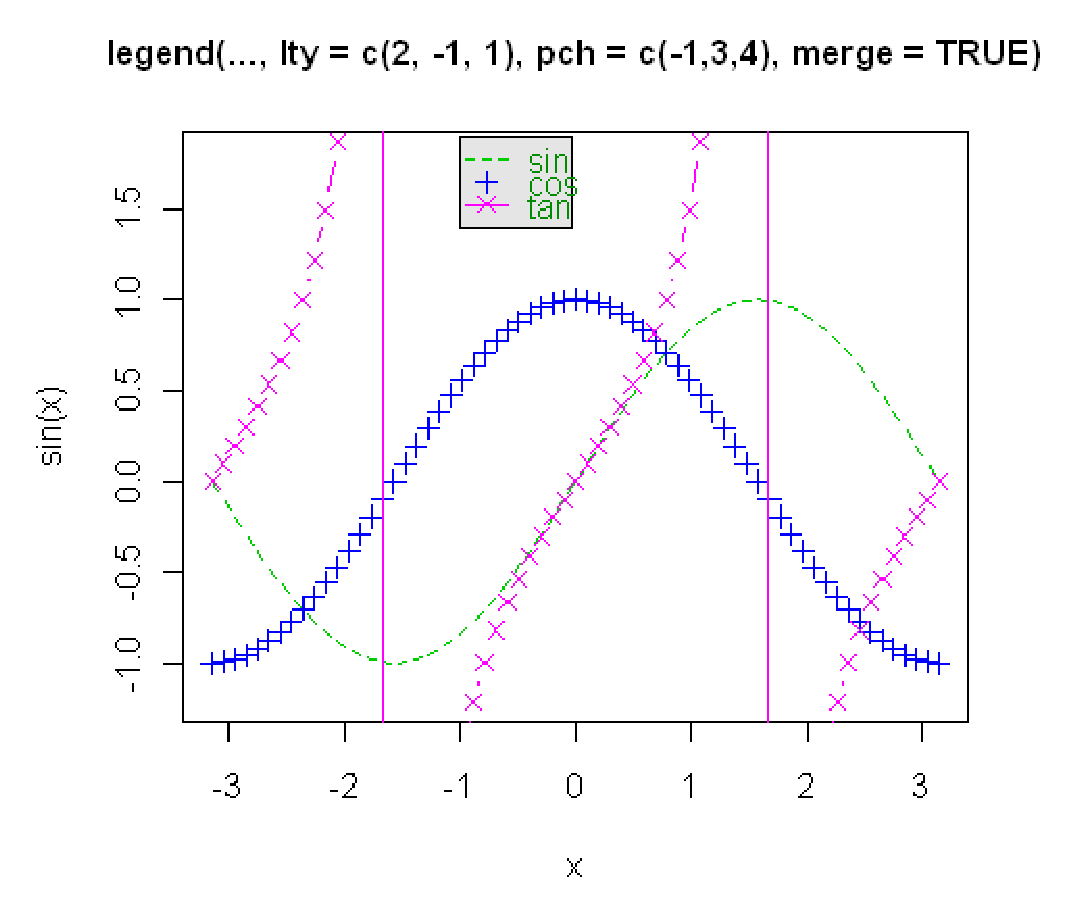
\includegraphics[height=5cm]{./images/legend.eps}}
\caption{Plot with a legend}
\label{fig:legend}
\end{figure}

If you don't know the location where to put the legend, you can use
the {\bf locator()} function which will return the coordinates where
you click the mouse. 

\subsection{Axis}
\label{sec:axis}

You can make any changes to axis (tick step, arrows, ...)
\begin{lstlisting}
axis(side, at = NULL, labels = TRUE, tick = TRUE, line = NA,
     pos = NA, outer = FALSE, font = NA, lty = "solid",
     lwd = 1, lwd.ticks = lwd, col = NULL, col.ticks = NULL,
     hadj = NA, padj = NA, ...)
\end{lstlisting}


\begin{itemize}
\item xpd=TRUE: normally, the tick at the far end are clipped at the plot region. So, if you want the tick at the far end to be drawn, enable this option
\end{itemize}

\subsection{A Box}
\label{sec:box}

You can add a box
\begin{lstlisting}
box()
\end{lstlisting}


\section{2D graphs}
\label{sec:2d-graphs}

\subsection{Boxplot}
\label{sec:boxplot}

There are two options: use the default function {\bf boxplot()} or the
function written in the {\it aplpack} package: {\bf boxplot2D()}

\begin{lstlisting}
boxplot(x, ..., range = 1.5, width = NULL, varwidth = FALSE,
        notch = FALSE, outline = TRUE, names, plot = TRUE,
        border = par("fg"), col = NULL, log = "",
        pars = list(boxwex = 0.8, staplewex = 0.5, outwex = 0.5),
        horizontal = FALSE, add = FALSE, at = NULL)
\end{lstlisting}
Visually display the summary of the distribution of the set of observations denoted by vector x.

Statistical issues:
\begin{itemize}
\item If we want to see how distribution of different variables in the
  same plot (e.g. there will be many box on the same plot), you need
  to group them with the function list() at the variable x 

\item range = this determines how far the plot whiskers extend out
  from the box (the values of zero causes the whisker extends to the
  data extremes \verb|->| there will be no outliers to be detected) 

\item plot = if FALSE, return the statistical summary of information
  from the plot, otherwise, return the plot 

\item notch = TRUE: draw the notch \verb|->| if the notches of two
  plots do not overlap this is 'strong evidence' that the two
  medians differ

\end{itemize}

Graphical issues:
\begin{itemize}
\item with = gives the relative width of the boxes making up the plot
varwidth is TRUE, the boxes are drawn with widths proportional to the
square-roots of the number of observations in the groups 

\item outline = to draw outline or not 

\item Add name to the graphs: set the parameter names
boxwex = scale all box \verb|->| improve visual performance when there
are a few box in the plot 

\item col = 

\item add = TRUE: add the boxplot to the current plot

\end{itemize}

{\bf Example}: 
\begin{lstlisting}
> boxplot(list(men, female), names = c("male", "female"))
\end{lstlisting}

NOTE: In the graph, points that are 'very extreme' are plotted by
themselves (outliers). Other data are represented


\section{Combine plots}
\label{sec:combine-plots}

\url{http://www.statmethods.net/advgraphs/layout.html}

%%% Local Variables: 
%%% mode: latex
%%% TeX-master: "R_language"
%%% End: 
